%\begin{minipage}[position]{width}
%text
%\end{minipage}
\subsection{Konfigurationsmenü 1 - Platz}\label{Konfig1}
\begin{wrapfigure}{l}{4.5cm}
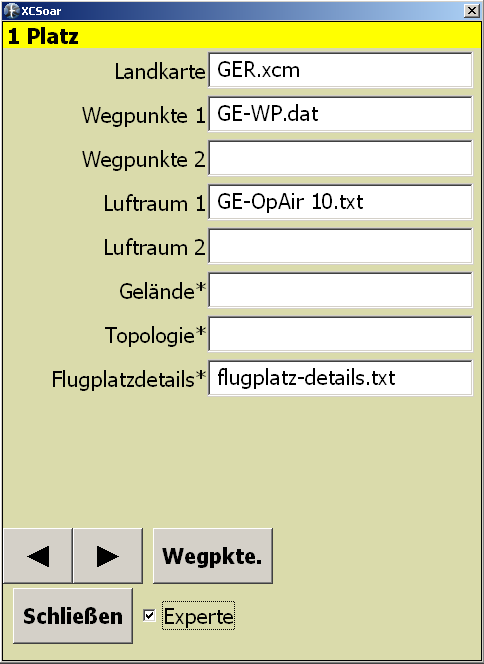
\includegraphics[width=4.5cm]{Bilder/Konfig1Platz.png}
\end{wrapfigure}
\textsf{Landkarte} Auswahl der Landkarte, welche benutzt werden soll. (\texttt{.xcm})-Format. Hierin enthalten ist bereits die Topologie mit Seen, Flüssen und Städten\\[0.5em]
\textsf{Wegpunkte 1} Wegpunktfile 1\\[0.5em]
\textsf{Wegpunkte 2} Ein zweites, optionales Wegpunktfile 2\\[0.5em]
\textsf{Luftraum 1} Luftraumfile 1, OpenAir-Format\\[0.5em]
\textsf{Luftraum 2} Luftraumfile 2, OpenAir-Format, ein zweites, optionales File\\[0.5em]
\textsf{Gelände$\ast$} Ein zweites, optionales  Geländefile \\[0.5em]
\textsf{Topologie$\ast$} Einzweites, optionales Topologiefile\\[0.5em]
\textsf{Flugplatzdetails$\ast$} Hierdrin stehen Details zu den Flugplätzen wie z.B. Bahnlänge, -belag, -richtung und z.B. Funkfreuqenz.


\button{Wegpkte.\ }\\[0.5em]
\textsf{Neu} Es öffnet sich eine Maske, auf der neue Wegpunkte bearbeitet/eingefügt werden können.\\[0.5em]
\textsf{Bearbeiten}] Maske zum Bearbeiten und ändern bereits vorhandene Wegpunkte.\\[0.5em]
\textsf{Speichern} Speichert die oben gemachten Änderungen.\\[0.5em]
\textsf{Löschen} Löscht den ausgewählten Wegpunkt

\subsection{Konfigurationsmenü 2 -Luftraum}\label{Konfig2}
\begin{wrapfigure}{r}{5.2cm}
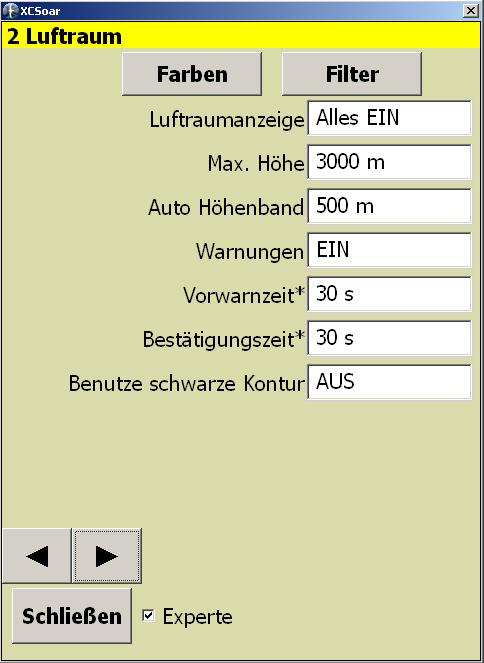
\includegraphics[width=4.5cm]{Bilder/Konfig2Luftraum.png}
\end{wrapfigure}
\begin{enumerate}
\item[Luftraumanzeige]
\item[Max.\ Höhe]
\item[Auto Höhenband]
\item[Warnungen]
\item[Vorwarnzeit$\ast$]
\item[Bestätigungszeit$\ast$]
\item[Benutze schwarze Kontur]
\end{enumerate}
\button{Farben} \qquad \button{Filter}

\subsection{Konfigurationsmenü 3 -Kartenanzeige}\label{Konfig3}
\begin{wrapfigure}{r}{5.2cm}
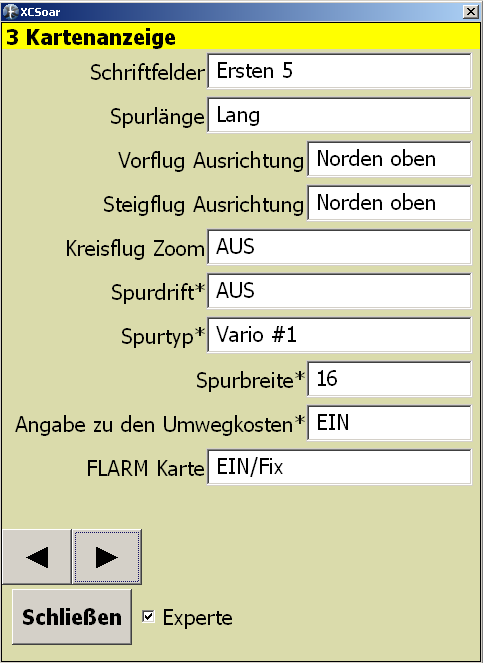
\includegraphics[width=4.5cm]{Bilder/Konfig3Kartenanzeige.png}
\end{wrapfigure}
\begin{enumerate}
\item[Schriftfelder]
\item[Spurlänge]
\item[Vorflug Ausrichtung]
\item[Steigflug Ausrichtung]
\item[Kreisflug Zoom]
\item[Spurdrift$\ast$]
\item[Spurtyp$\ast$]
\item[Spurbreite$\ast$]
\item[Angabe zu den Umwegkosten$\ast$]
\item[FLARM Karte]

\end{enumerate}

\subsection{Konfigurationsmenü 4 - Kartensymbole}\label{Konfig4}
\begin{wrapfigure}{r}{5.2cm}
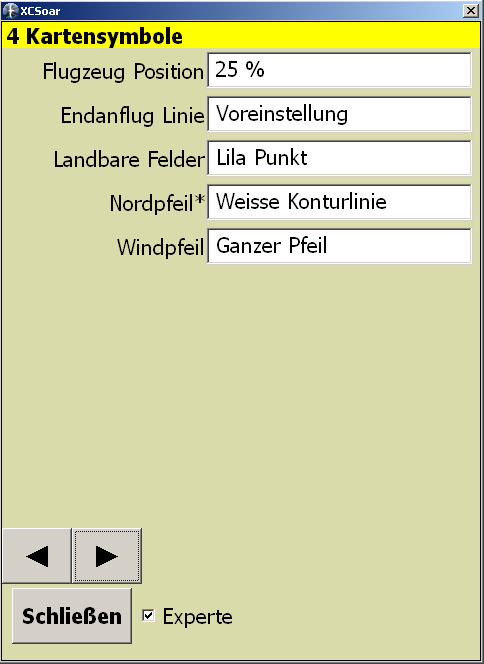
\includegraphics[width=4.5cm]{Bilder/Konfig4Kartensymbole.png}
\end{wrapfigure}
\begin{enumerate}
\item[Flugzeug Position]
\item[Endanflug Linie]
\item[Landbare Felder]
\item[Nordpfeil$\ast$]
\item[Windpfeil]
\end{enumerate}

\subsection{Konfigurationsmenü 5 - Gelände Anzeige}\label{Konfig5}
\begin{wrapfigure}{r}{5.2cm}
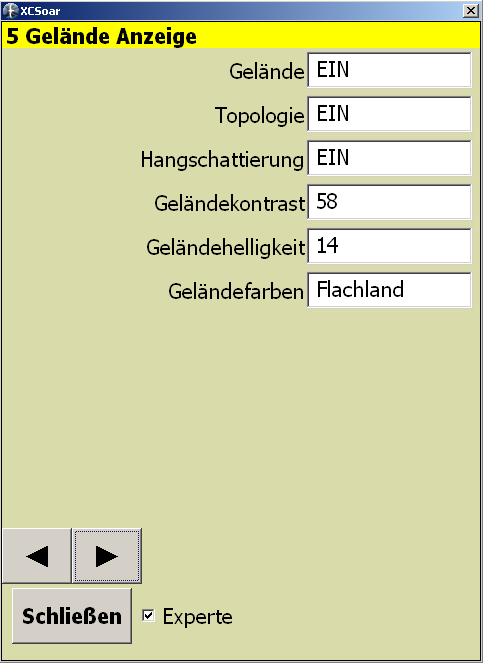
\includegraphics[width=4.5cm]{Bilder/Konfig5Gelaendeanzeige.png}
\end{wrapfigure}
\begin{enumerate}
\item[Gelände]
\item[Topologie]
\item[Hangschattierung]
\item[Geländekontrast]
\item[Geländehelligkeit]
\item[Geländefarben]
\end{enumerate}

\subsection{Konfigurationsmenü 6 - Endanflugrechner}\label{Konfig6}
\begin{wrapfigure}{r}{5.2cm}
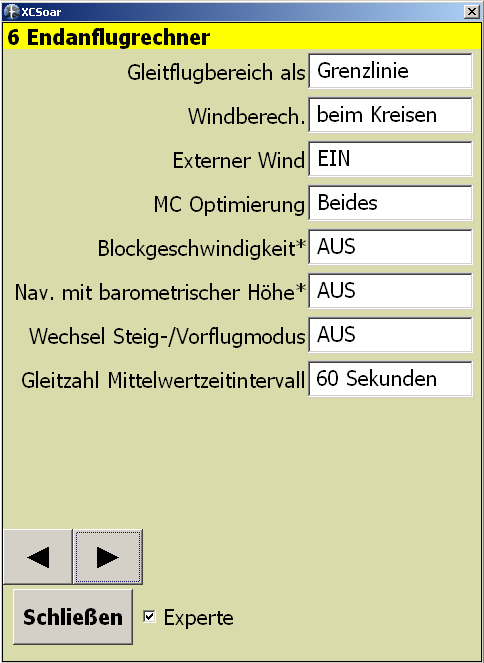
\includegraphics[width=4.5cm]{Bilder/Konfig6Endanflugrechner.png}
\end{wrapfigure}
\begin{enumerate}
\item[Gleitflugbereich als] Einstellung, wie der aktuelle Gleitbereich dargestellt werden soll: \textsf{Off} Keine Darstellung des Gleitbereiches. \textsf{Grenzlinie} Eine Linie wird um das Flugzeug gezeichnete welches den Gleitbereich darstellt. \textsf{Schattiert}: Außerhalb des Gleitbereiches wird der Bildschirm schattiert dargestellt.
\item[Windberech.]Einstellungen zur Berechnung des Windes: \textsf{ Manuell}: Der Pilot ist verantwortlich für die Eingabe des Windes. Keine automatische Berechnung \textsf{ beim Kreisen}Wind wird beim Kreisen durch Windversatz anhand GPS-Quelle ermittelt. \textsf{ZickZack}Wind kann  mithilfe eines intelligenten Variometers  errechnet werden, welches die IAS auszugeben in der Lage ist \textsf{Beides} Es werden beide vorher genannten Möglichkeiten zur Berechnung herangezogen.
\item[Externer Wind] Ein/Aus. Wenn eingeschaltet, wird der Wind von externen Geräten zur Berechnung heran- und der von \xc vorgezogen.
\item[MC Optimierung]\textsf{Endandflug} \textsf{Erwartetes mittleres Steigen} \textsf{Beides}
\item[Blockgeschwindigkeit$\ast$] Wenn aktiviert, wird im
Vorflug diejenige \textsf{MC} - Geschwindigkeit vorgeschlagen,  die für den Flug \textsl{ohne} vertikale Luftbewegung gilt. Andernfalls wird die \textsf{Delphin-Stil} Vorfluggeschwindigkeit vorgeschlagen.

    D.h.\ die \textsf{MC}-Geschwindigkeit, welche unter Berücksichtigung der vertikalen Luftmassenbewegung gilt.
\item[Nav.\ mit barometrischer Höhe$\ast$] Wenn aktiviert und vorhanden, wird die barometrische Höhe aus einem externen Gerät für alle Navigationsfunktionen verwendet.  Andernfalls wird die \textsf{GPS}-Höhe verwendet.
\item[Wechsel Steig/Vorflugmodus] \textsf{Aus} Wenn aus, dann manuell oder wie ???  \textsf{Wölbklappe} Wenn VEGA Vario und Wölbklappe gewählt ist, wird mit der Wölbklappe zwischen Kreis- und Vorflug umgeschaltet  \textsf{ man.\ Schalter} Schalter an Wölbklappe oder externer Schalter schaltet um\stop
\item[Gleitzahl Mittelwert-Zeitintervall]Zeit zur Berechnung des Mittelwertes der Gleitzahl.\footnote{Ausführliche  Beschreibung folgt später.} Standard 90sec.\
\end{enumerate}

\subsection{Konfigurationsmenü 7 - Sicherheitsfaktoren}\label{Konfig7}
\begin{wrapfigure}{r}{5.2cm}
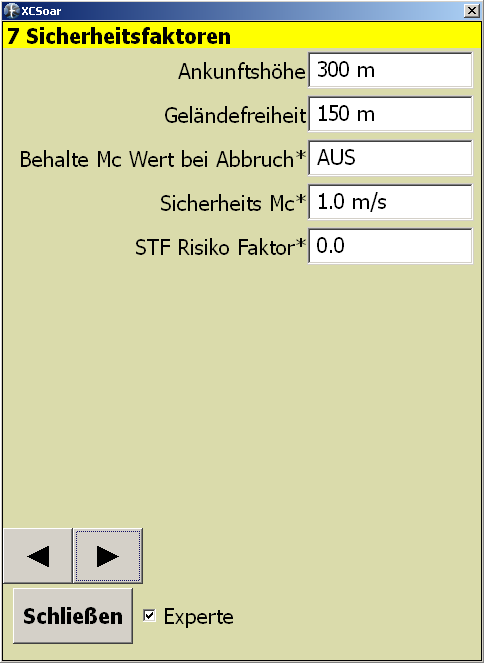
\includegraphics[width=4.5cm]{Bilder/Konfig7Sicherheistfaktoren.png}
\end{wrapfigure}
\begin{enumerate}
\item[Ankunftshöhe]
\item[Geländefreiheit]
\item[Behalte \textsf{MC} Wert bei Abbruch$\ast$]
\item[Sicherheits \textsf{MC}$\ast$]
\item[STF Sicherheitsfaktor$\ast$]
\end{enumerate}


\subsection{Konfigurationsmenü 8 - Polare}\label{Konfig8}
\begin{wrapfigure}{r}{5.2cm}
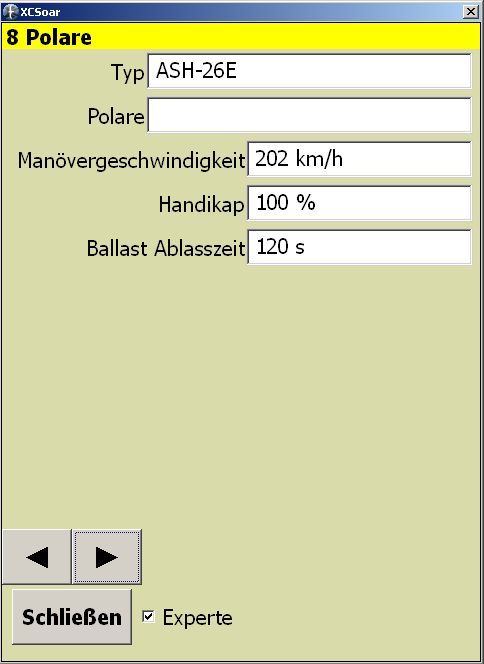
\includegraphics[width=4.5cm]{Bilder/Konfig8Polare.png}
\end{wrapfigure}
\begin{enumerate}
\item[Typ] Auswahl aus einer internen Liste möglich
\item[Polare] Wenn hier eine externe Polare gewählt werden soll, dann muß in diesem Feld die Datei mit der Polaren im \textsf{WinPilot}-Format angegeben werden.
\item[Mannövergeschwindigkeit] Auswahl der zulässigen Mannövergeschwindigkeit des gewählten Flugzeuges
\item[Handikap] Handicap - Faktor für die \textsf{OLC}-Wettbewerb Wertung
\item[Ballast Ablaßzeit] Benötigte Zeit zum kompletten Ablassen des Wasserballastes
\end{enumerate}


\subsection{Konfigurationsmenü 9 - NMEA-Anschluß (GPS-Quelle)}\label{Konfig9}
\begin{wrapfigure}{r}{5.2cm}
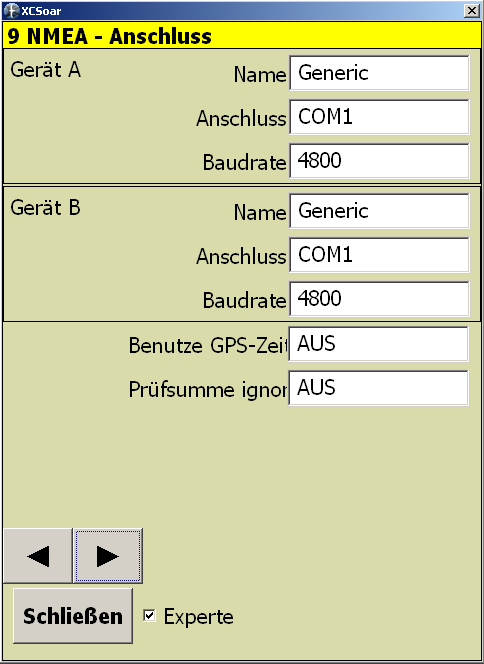
\includegraphics[width=4.5cm]{Bilder/Konfig9NMEAAnschluss.png}
\end{wrapfigure}
\begin{enumerate}
\item[Gerät A]
\begin{itemize}
\item[Name] Typ der primär angeschlossenen \textsf{GPS}-Quelle. Es sollte die zuverlässigste Quelle an Bord sein.
\item[Anschluß] Auswahl des COM-Ports. Benutzer des \textsf{Altair} müssen diesen Anschluß auf COM 3 stellen!
\item[Baudrate]\textsf{Altair} und \textsf{Vega} Benutzer sollten diese Einstellung auf 38400 stellen.
\end{itemize}
\item[Gerät B]
\begin{itemize}
\item[Name] Typ des zusätzlichen Gerätes. Es kann ein Ersatz-GPS, oder auch für andere Daten z.B.\ ein intelligentes Variometer sein.
    "Generisch" ist de Einstellung für eine \textsf{GPS}-Quelle, FLARM eingeschlossen.
\item[Anschluß]Auswahl des COM-Ports.  Benutzer des \textsf{Altair} müssen diesen Anschluß auf COM 1 stellen!
\item[Baudrate]\textsf{Altair} und \textsf{Vega} Benutzer sollten diese Einstellung auf 38400 stellen.
\end{itemize}
\item[Benutze \textsf{GPS}-Zeit]
\item[Prüfsumme ignorieren$\ast$]
\end{enumerate}



\subsection{Konfigurationsmenü 10 - Maßeinheiten}\label{Konfig10}
\begin{wrapfigure}{r}{5.2cm}
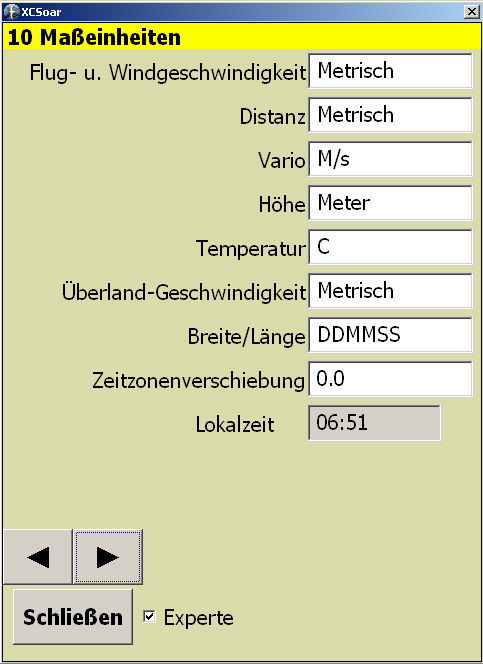
\includegraphics[width=4.5cm]{Bilder/Konfig10Masseinheiten.png}
\end{wrapfigure}
\begin{enumerate}
\item[Flug- u.\ Windgeschwindigkeit]
\item[Distanz]
\item[Vario]
\item[Höhe]
\item[Temperatur]
\item[Überland-Geschwindigkeit]
\item[Breite/Länge]
\item[Zeitzonenverschiebung]
\item[Lokalzeit]
\end{enumerate}

\subsection{Konfigurationsmenü 11 - Benutzeroberfläche}\label{Konfig11}
\begin{wrapfigure}{r}{5.2cm}
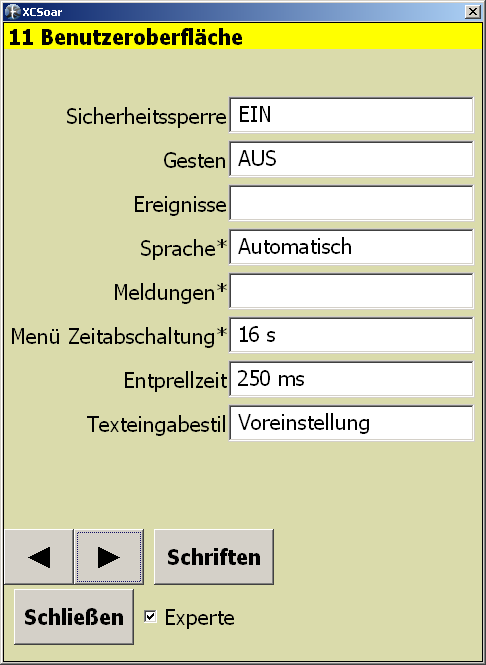
\includegraphics[width=4.5cm]{Bilder/Konfig11BenutzerOF.png}
\end{wrapfigure}
Hier erfolgt die Einstellung der Benutzer Oberfläche sowie die Auswahl der Schriften für diverse Menüs, labels etc.\
\begin{center}
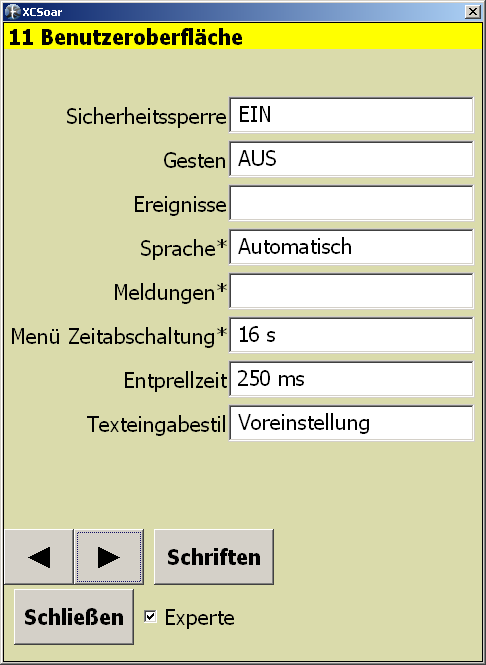
\includegraphics[width=11cm]{Bilder/Konfig11BenutzerOF.png}
\end{center}
\begin{enumerate}
\item[Sicherheitssperre:]  Ein/AUS
Einstellung, ob das Konfigurationsmenü während des Fluges  erreichbar sein soll. (Stört und macht unaufmerksam.)
\item[Gesten:] Ein/Aus
Einstellung, ob \xc auch mit Gesten auf dem Touchscreen gesteuert werden können soll
\item[Ereignisse:] Eine mögliche Eingabe-Ereignisdatei bestimmt das Menüsystem und wie \xc auf einem Knopfdruck oder z.B.\ auf ein Ereignis eines anderen externen Gerätes reagieren soll.
\item[Sprache$\ast$:] Hier wird die gewünschte Menüsprache gewählt. Es ist keine externe Sprachdatei mehr notwendig und möglich.
\item[Meldungen$\ast$:] Hier kann eine Datei angegeben werden, in festgelegt wird, welche Klänge wann und wie lange bei bestimmten Ereignissen abgespielt werden sollen.
\item[Menü Zeitabschaltung$\ast$:] Legt fest, wie lange ein Menü angezeigt wird, wenn der Benutzer keine Eingabe macht.
\item[Entprellzeit:]Minimale Zeit, nach der das System einen erneuten Tastendruck als Eingabe akzeptiert. Hilft, falls Tasten klemmen oder prellen.
\item[Texteingabestil:] Voreinstellung/Tastatur/Ranglisten Stil.
Vorgabe: Tastatur.\\
Tastatur: Inkrementelle Suche - Schnell und unkompliziert.

Ranglisten Stil: Eingabe mittels Cursorpfeilen (rechts-links, hoch-runter) entsprechende Buchstabe gefunden ist.
\end{enumerate}



\subsection{Konfigurationsmenü 12 - Anordnung}\label{Konfig12}
\begin{wrapfigure}{r}{5.2cm}
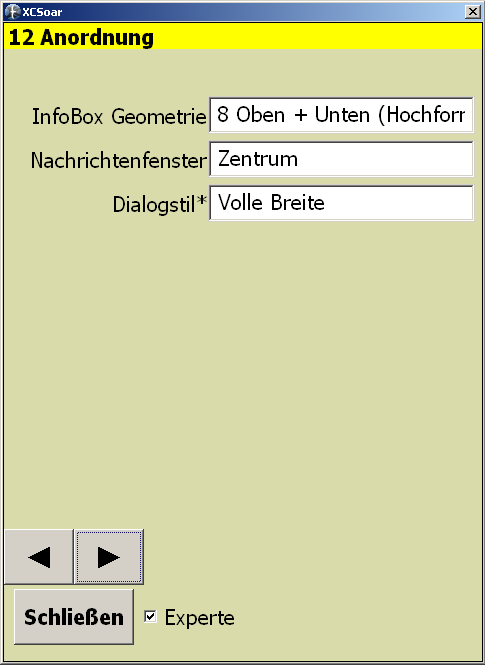
\includegraphics[width=4.5cm]{Bilder/Konfig12Anordnung.png}
\end{wrapfigure}

\begin{enumerate}
\item[Infobox Geometrie]
\item[Nachrichten Fenster $\ast$]
\item[Dialogstil $\ast$]
\end{enumerate}

\subsection{Konfigurationsmenü 13 - Flarm und andere Anzeigen}\label{Konfig13}
\begin{wrapfigure}{r}{5.2cm}
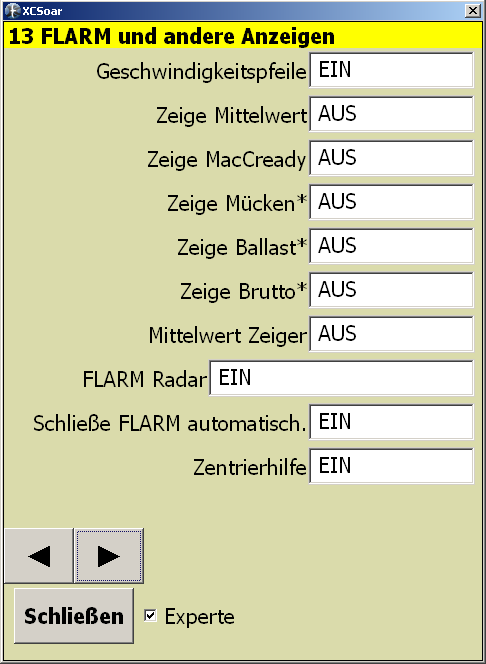
\includegraphics[width=4.5cm]{Bilder/Konfig13FLARM.png}
\end{wrapfigure}
\begin{enumerate}
\item[Geschwindigkeitspfeile]
\item[Zeige Mittelwert]
\item[Zeige Mc Cready-Wert]
\item[Zeige Mücken]
\item[Zeige Ballast]
\item[Zeige Brutto]
\item[Mittelwert Zeiger]
\item[Flarm Radar]
\item[Schließe FLARM automatisch]
\item[Zentrierhilfe]
\end{enumerate}

\subsection{Konfigurationsmenü 14 - Standard Wettbewerbsregeln}\label{Konfig14}
\begin{wrapfigure}{r}{5.2cm}
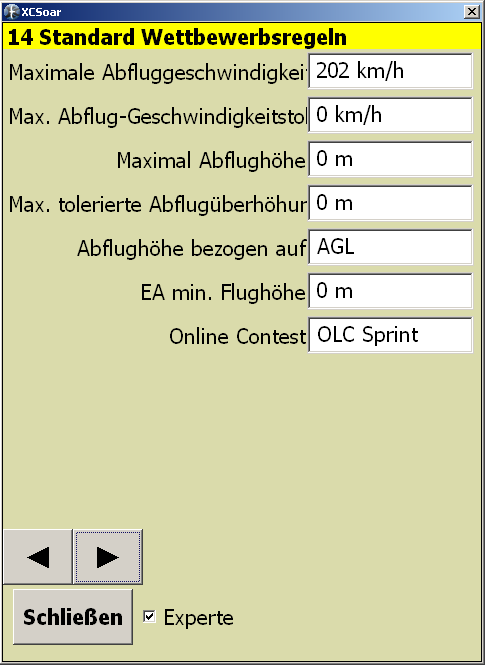
\includegraphics[width=4.5cm]{Bilder/Konfig14Wettbewerb.png}
\end{wrapfigure}
\begin{enumerate}
\item[Maximale Abfluggeschwindigkeit]
\item[Max.\ Abflug-Geschwindigkeitstoleranz]
\item[Maximale Abflughöhe]
\item[Max.\  tolerierte Abflughöhung ]
\item[Abflughöhe bezogen auf]
\item[EA min.\ Flughöhe]
\item[Online Contest]
\end{enumerate}

\subsection{Konfigurationsmenü 15 - Infoboxen}\label{Konfig15}
\begin{wrapfigure}{r}{5.2cm}
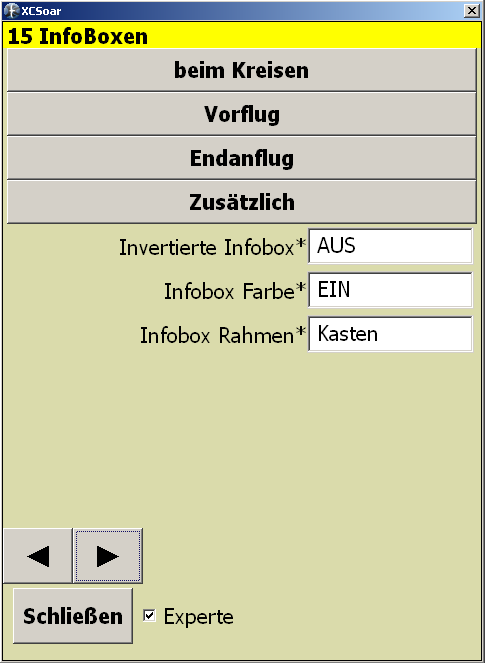
\includegraphics[width=4.5cm]{Bilder/Konfig15Infoboxen.png}
\end{wrapfigure}
\begin{enumerate}
\item[beim Kreisen]
\item[Vorflug]
\item[Invertierte Infobox$\ast$]
\item[Infobox Farbe$\ast$]
\item[Zusätzlich$\ast$]
\end{enumerate}

\subsection{Konfigurationsmenü 16 - Logger}\label{Konfig16}
\begin{wrapfigure}{r}{5.2cm}
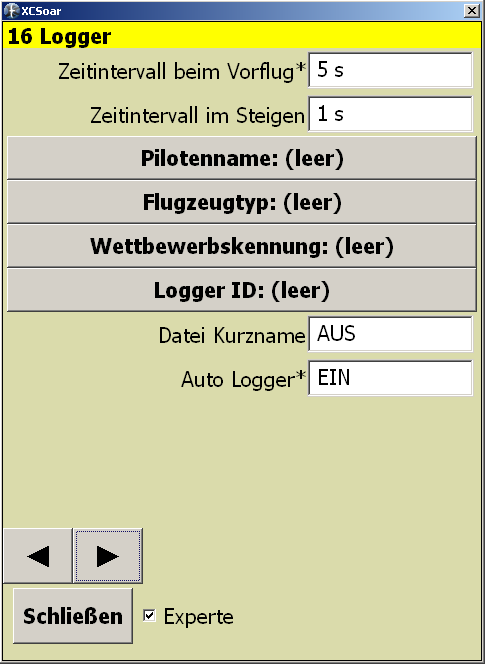
\includegraphics[width=4.5cm]{Bilder/Konfig16Logger.png}
\end{wrapfigure}
\begin{enumerate}
\item[Zeitintervall beim Vorflug$\ast$]
\item[Zeitintervall beim Steigen]
\item[Pilotenname]
\item[Flugzeugtyp]
\item[Wettbewerbskennung]
\item[Logger ID]
\item[Datei Kurzname] Der Loggerschrieb des Fluges wird in eine Datei geschrieben
Diese Einstellung legt fest, ob kurze oder lange IGC-Dateinamen verwendet werden:
Kurz: 81HXABC1.IGC,  Lang: 2008-01-18-XXX-ABC-01.IGC
\item[Auto Logger$\ast$] Aktiviert den automatischen Loggerschrieb beim Abheben und Landen. Achtung: Bei Gleitschirmen muß dies Feld auf Aus stehen, da die Geschwindigkeiten i.d.R.\ zu gering sind.
\end{enumerate}

\subsection{Konfigurationsmenü 17 - Experimental}\label{Konfig17}
\begin{wrapfigure}{r}{5.2cm}
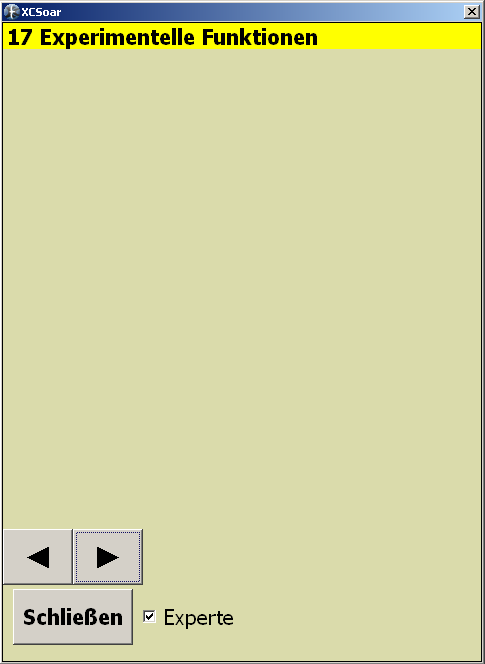
\includegraphics[width=4.5cm]{Bilder/Konfig17Experimental.png}
\end{wrapfigure}
\begin{enumerate}
\item[Bisher ohne Funktion]
\end{enumerate} 